\documentclass[12pt,letterpaper, onecolumn]{exam}
\usepackage{amsmath}
\usepackage{amssymb}
\usepackage{listings}
\usepackage{hyperref}
\usepackage{xcolor}
\usepackage{bookmark}
\usepackage{graphicx}
\newcommand{\link}[1]{{\color{blue}\href{#1}{#1}}}
\usepackage{pythonhighlight}
\usepackage[a4paper,lmargin=30pt, rmargin=50pt, tmargin=0.65in]{geometry}  %For centering solution box
% \chead{\hline} % Un-comment to draw line below header
\thispagestyle{empty}   %For removing header/footer from page 1

\begin{document}

\begingroup
\centering
\LARGE CS 474\\
\large Assignment 2 \\[0.5em]
\endgroup
\begingroup
\normalsize \quad\quad\quad Name: Adharsh Kamath \quad\quad\quad \quad\quad\quad \quad\quad\quad \quad\quad\quad \quad  NetID: ak128 \par\
\endgroup
\rule{17cm}{0.4pt}
\pointsdroppedatright   %Self-explanatory
\printanswers
\renewcommand{\solutiontitle}{\noindent\textbf{Soln:}\enspace}
\newcommand{\cheading}[1]{{\underline{\textit{#1}}}}

\renewcommand{\questionshook}{%
	\setlength{\leftmargin}{18pt}%
	\setlength{\labelwidth}{-\labelsep}%
}
\qformat{\underline{Problem \thequestion}}
\begin{questions}
	\question[]
	\solutiontitle

	Let us use the symbol $\psi$ to refer to the given formula.
	\begin{align*}
		\psi = \left( p \land  (p \Rightarrow q) \right) \Rightarrow q
	\end{align*}

	In order to show that $\psi$ is valid, we can show that 
	\begin{align*}
		\neg \psi = \neg \left( (p \land  (p \Rightarrow q)  \Rightarrow q) \right)
	\end{align*}
	is unsatisfiable. Rewriting the above formula:
	\begin{align*}
		\neg \psi = \neg \left( (p \land  (p \Rightarrow q)  \Rightarrow q) \right) \\
					\equiv \neg \left( (p \land  (\neg p \lor q) ) \Rightarrow q \right) \\
					\equiv \neg \left( \neg (p \land  (\neg p \lor q) ) \lor q \right) \\
					\equiv (p \land  (\neg p \lor q) ) \land \neg q
	\end{align*}

	The last step is due to De Morgan's Law. We can now convert this to CNF, and construct a resolution refutation to show that it is unsatisfiable.
	To convert to CNF, we use the Tseitin transformation. We only need three new propositional variables, $x_{\psi}, x_1, x_2$,
	where $x_{\psi}$ corresponds to $\psi$, $x_1$ corresponds to $(\neg p \lor q)$ and $x_2$ corresponds to $(p \land x_1)$.
	This gives us the following set of clauses:
	\begin{align*}
		\left .
			\begin{cases}
					\{ \neg x_{\psi} \}, \\
					\{ \neg \neg x_{\psi}, x_2 \}, \{ \neg \neg x_{\psi}, \neg q \}, \{ \neg x_{\psi}, \neg x_2, \neg \neg q \} \\
					\{ \neg x_2, p \}, \{ \neg x_2, x_1 \}, \{ x_2, \neg p, \neg x_1  \}, \\
					\{ x_1, \neg \neg p \}, \{ x_1, \neg q \}, \{ \neg x_1, \neg p, q \}, 
			\end{cases}
		\right\}
	\end{align*}

	Simplifying the set by replacing $ \neg \neg p $ with $ p $ for all propositional variables $p$, we get:
	\begin{align*}
		\left .
			\begin{cases}
				\{ \neg x_{\psi} \}, \\
				\{ x_{\psi}, x_2 \}, \{ x_{\psi}, \neg q \}, \{ \neg x_{\psi}, \neg x_2, q \} \\
				\{ \neg x_2, p \}, \{ \neg x_2, x_1 \}, \{ x_2, \neg p, \neg x_1  \}, \\
				\{ x_1, p \}, \{ x_1, \neg q \}, \{ \neg x_1, \neg p, q \},
			\end{cases}
		\right\}
	\end{align*}

	We can now create a resolution refutation to show that this set is unsatisfiable:
	\begin{align*}
		& 1. \{ \neg x_{\psi} \} \\
		& 2. \{ x_{\psi}, x_2 \} \\
		& 3. \{ x_2 \} \quad \text{Resolvent of 1 and 2} \\
		& 4. \{ \neg x_2, p \} \\
		& 5. \{ p \} \quad \text{Resolvent of 3 and 4} \\
		& 6. \{ \neg x_1, \neg p, q \} \\
		& 7. \{ \neg x_1, q \} \quad \text{Resolvent of 5 and 6} \\
		& 8. \{ x_{\psi}, \neg q \} \\ 
		& 9. \{ x_{\psi}, \neg x_1 \} \quad \text{Resolvent of 7 and 8} \\
		& 10. \{ \neg x_1 \} \quad \text{Resolvent of 1 and 9} \\
		& 11. \{ \neg x_2, x_1 \} \\
		& 12. \{ x_1 \} \quad \text{Resolvent of 3 and 11} \\
		& 13. \{  \} \quad \text{Resolvent of 10 and 12}
	\end{align*}

	By creating this resolution refutation, we have shown that there is no valuation that can satisfy $ \neg \psi $.
	Since $ \neg \psi $ is unsatisfiable, we can conclude that $ \psi $ is valid.

	The above proof can be validated using the resolution tool provided as a part of the assignment.
	The initial set of clauses, and the resulting resolution proof object can be found at 
	\link{https://github.com/adharshkamath/cs474-hw/tree/main/resolution\_proofs/p1}

    {\rule{17cm}{0.4pt}}
	\question[]
	\solutiontitle

	We are given the formula:
	\begin{align*}
		\psi = (q \lor \neg r) \land (\neg p \lor r) \land (\neg q \lor r \lor p) \land (p \lor q \lor \neg q) \land (\neg r \lor q)
	\end{align*}

	The set of clauses representing this formula is:
	\begin{align*}
		\left .
			\begin{cases}
				\{q, \neg r\}, \{\neg p, r\}, \{\neg q, r, p\}, \{p, q, \neg q\}, \{\neg r, q\}
			\end{cases}
		\right\}
	\end{align*}

	\textbf{(a):}

	We shall consider resolutions that (i) lead to new clauses and are (ii) not trivial. 
	For example, resolving $\{q, \neg r \}$ and $\{ \neg q, r \lor p \}$ gives us $\{ r, \neg r, p \}$, which is trivially true and hence not included
	in the resolution steps below. we will use the given formula as is, without modifying the given formula (removing any trivial or redundant conjuncts).  
	
	We can find resolvents in the following way:
	\begin{align*}
		& 1. \{ q, \neg r \} \\
		& 2. \{ \neg p, r \} \\
		& 3. \{ q, \neg p \} \quad \text{Resolvent of 1 and 2} \\
		& 4. \{ p, q, \neg q \} \\
		& 5. \{ p, q, \neg r \} \quad \text{Resolvent of 1 and 4} \\
		& 6. \{ \neg q, r, p \} \\
		& 7. \{ r, \neg q \} \quad \text{Resolvent of 2 and 6}
	\end{align*}

	The final set of clauses is:
	\begin{align*}
		\left .
			\begin{cases}
				\{q, \neg r\}, \{\neg p, r\}, \{\neg q, r, p\}, \{p, q, \neg q\}, \{\neg r, q\} \\
				\{ q, \neg p \}, \{ p, q, \neg r \}, \{ r, \neg q \}
			\end{cases}
		\right\} \quad \quad (1) \label{set1}
	\end{align*}

	Note that, if we had removed redundant and trivial clauses from the initial set of clauses, the final set would be different in the following ways:
	\begin{itemize}
		\item The clause $\{ p, q, \neg q \} $ would be removed since it is trivial
		\item The clause $\{ \neg r, q \}$ would be removed since it is redundant
		\item The resolvent $ \{ p, q, \neg r \} $ would not be present in the final set since $\{ p, q, \neg q \} $ was removed from the initial set (step 4 in the resolution)
	\end{itemize}

	The final set of clauses in that case would be:
	\begin{align*}
		\left .
			\begin{cases}
				\{q, \neg r\}, \{\neg p, r\}, \{\neg q, r, p\}, \\
				\{ q, \neg p \}, \{ r, \neg q \}
			\end{cases}
		\right\}
	\end{align*}

	These initial and final sets can be observed in the interaction with the resolution tool. The tool discards trivial and redundant clauses before the resolution steps are entered. \\
	

	\textbf{(b):}

	Encoding the initial formula using the python library for Z3:

	\begin{python}
from z3 import *

p = Bool("p")
q = Bool("q")
r = Bool("r")

s = Solver()

s.add(
	(And 
		(Or(q, Not(r))),
		(Or(Not(p), r)),
		(Or(Not(q), r, p)), 
		(Or(p, q, Not(q))), 
		(Or (Not (r), q)),
	)
)


print(s.check())
print(s.model())
	\end{python}

	The following output can be observed when the above program is executed:
\begin{lstlisting}
sat
[q = False, p = False, r = False]
\end{lstlisting}
As we can see, the formula is satisfiable and Z3 finds a satisfying valuation, where all $p, q, r$ are set to $\text{false}$.

In order to show the equivalence of $ \varphi $, the initial set of clauses, and $ \psi $ the final set, we can show the unsatisfiability of 
$ \neg (\varphi \leftrightarrow \psi) $. This would mean that $ (\varphi \leftrightarrow \psi) $ is valid. Below is the program for the same:
\begin{python}
from z3 import *

p = Bool("p")
q = Bool("q")
r = Bool("r")

s = Solver()

s.add(
	Not(
		(
			And(
				(Or(q, Not(r))),
				(Or(Not(p), r)),
				(Or(Not(q), r, p)),
				(Or(p, q, Not(q))),
				(Or(Not(r), q)),
			)
		)
		== (
			And(
				(Or(q, Not(r))),
				(Or(Not(p), r)),
				(Or(Not(q), r, p)),
				(Or(p, q, Not(q))),
				(Or(Not(r), q)),
				(Or(q, Not(p))),
				(Or(p, q, Not(r))),
				(Or(r, Not(q))),
			)
		)
	)
)

if s.check() == unsat:
	print("Formula valid!")
else:
	print("Formula not valid")
\end{python}

The following output is observed when the above program is executed:
\begin{lstlisting}
Formula valid!
\end{lstlisting}

Therefore, we can conclude that the sets of clauses $ \varphi $ and $ \psi $ are equivalent. 

The resolution steps in \textbf{(a)} can be performed using the resolution tool as well.
The initial set of clauses, and the resulting resolution proof object can be found at:

\link{https://github.com/adharshkamath/cs474-hw/tree/main/resolution\_proofs/p2}.

The Z3 code files mentioned previously can also be found in the same folder above.


    {\rule{17cm}{0.4pt}}
	\question[]
	\solutiontitle

	Since there is no restriction specified on the variable order, let us use the following order: 
	
	$ x_{\psi} > x_2 > q > x_1 > p $ 

	Constructing the decision tree with the above variable order gives us the following:

	\begin{center}
	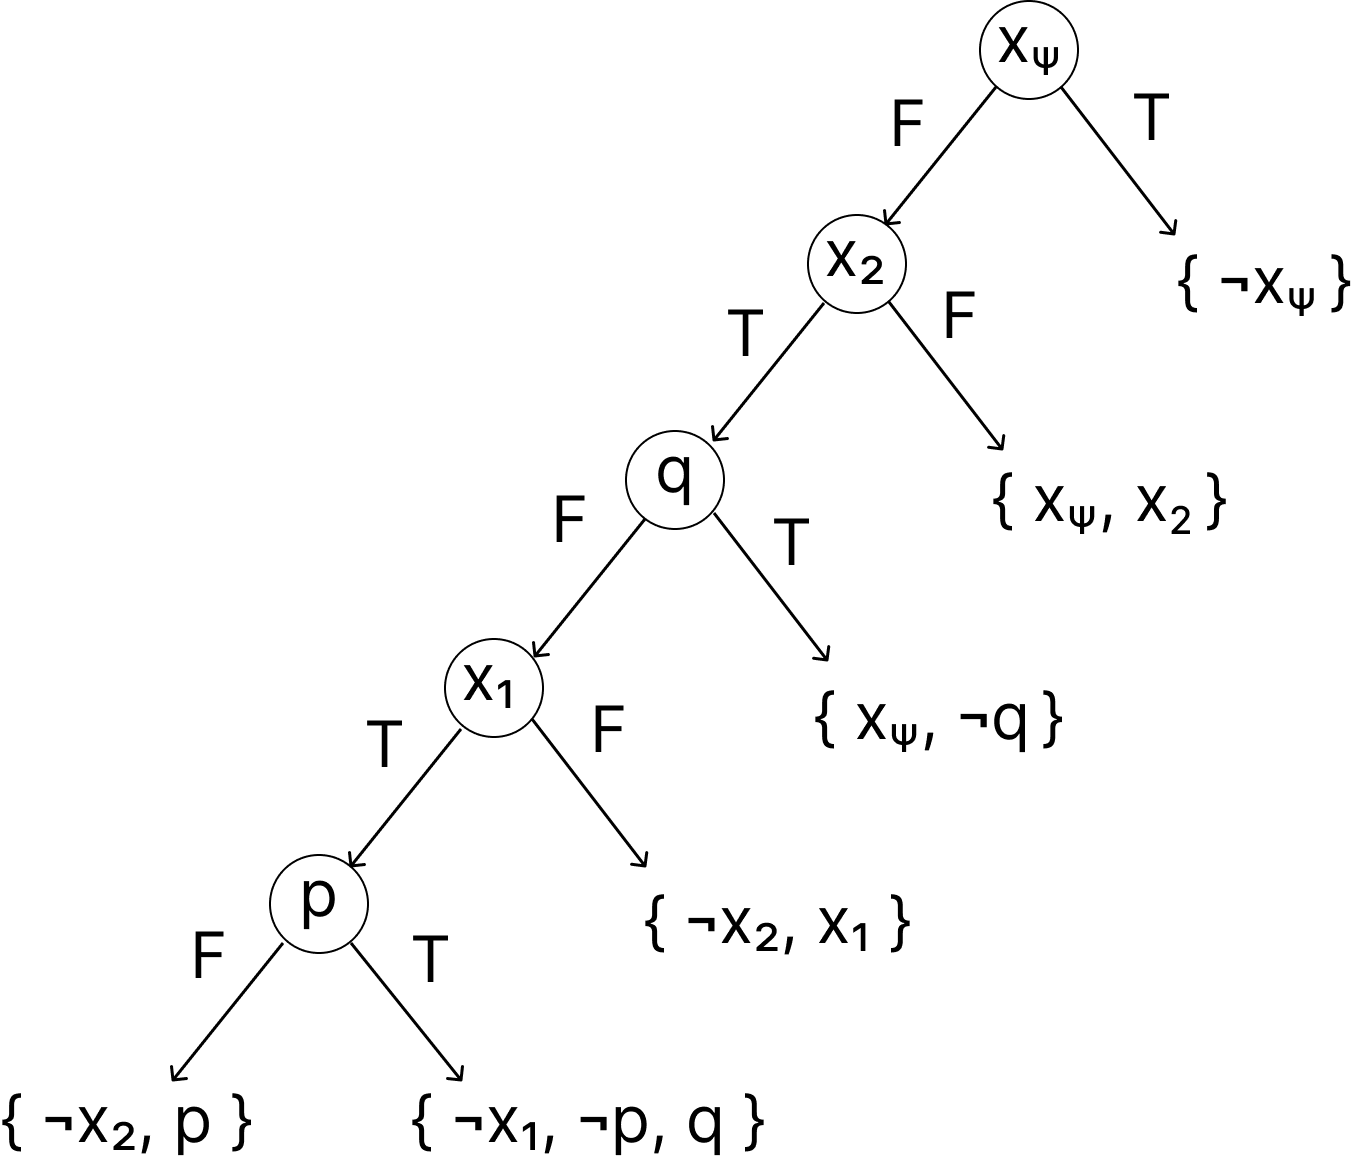
\includegraphics[scale=0.22]{decision_tree.png}
	\end{center}

	As we can see, all the paths are "blocked" and hence there is no satisfying assignment of values to the variables.
	We can obtain a resolution proof from the above tree in the following way:

	\begin{itemize}
		\item Take the children of node $ p $, $ \{ \neg x_2, p \} $ and $ \{\neg x_1, \neg p, q \} $ and resolve them on $ p $ to obtain  $ \{\neg x_2, \neg x_1, q \} $
		\item Now the left child of $ x_1 $ is $ \{\neg x_2, \neg x_1, q \} $ and the right child is $ \{ \neg x_2, x_1 \} $. Resolve them on $ x_1 $ to get $ \{ \neg x_2, q \} $
		\item Now the left child of $ q $ is $ \{ \neg x_2, q \} $ and the right child is $ \{ x_{\psi}, \neg q \} $. Resolve them on $ q $ to get $ \{ \neg x_2, x_{\psi} \} $
		\item Now the left child of $ x_2 $ is $ \{ \neg x_2, x_{\psi} \} $ and the right child is $ \{ x_2, x_{\psi} \} $. Resolve them on $ x_2 $ to get $ \{ \neg x_{\psi} \} $
		\item Finally, the left child of $ x_{\psi} $ is $ \{ \neg x_{\psi} \} $ and the right child is $ \{ x_{\psi} \} $. Resolve them on $ x_{\psi} $ to get $ \{  \} $
	\end{itemize}

	This proof can be viewed as follows:


	\begin{center}
	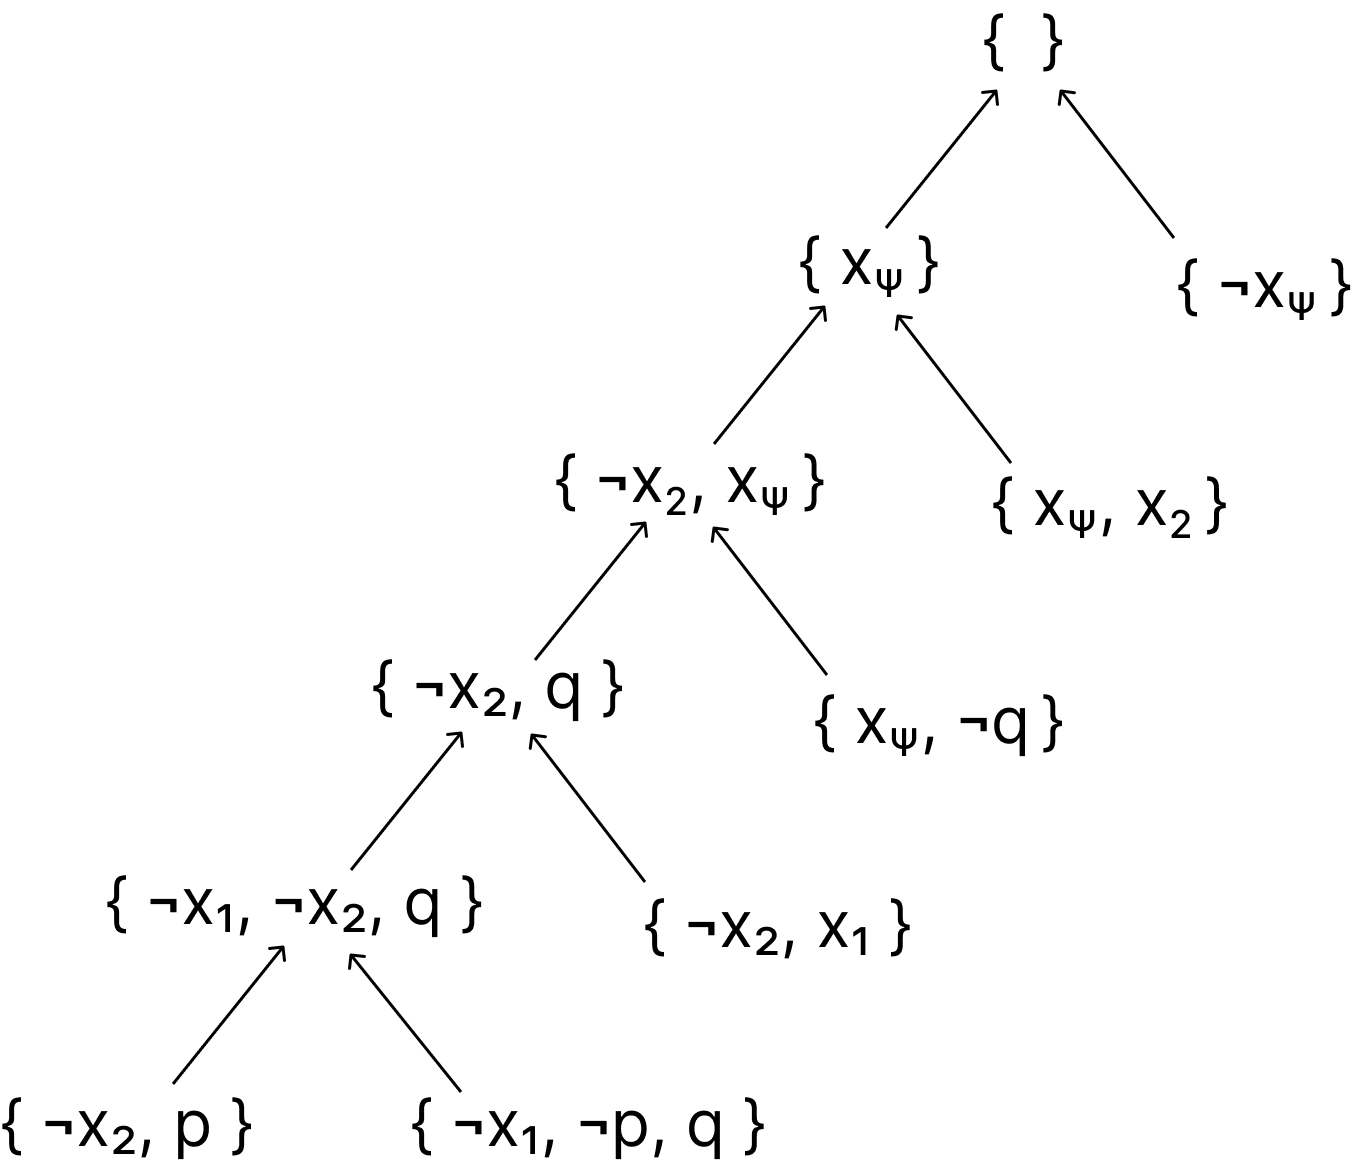
\includegraphics[scale=0.22]{resolution_proof.png}
	\end{center}


    {\rule{17cm}{0.4pt}}

\end{questions}
\end{document}